\section{Aggregation and Deaggregation Strategies}
\label{sec:agdag}

One of the primary drawbacks of Algorithm~\ref{alg:algoHybrid} is in handling the discrete transitions. 
%
Suppose that in a given location, the number of stars that overlap with the guard of a discrete transition (line~\ref{ln:guardIntersection} in Algorithm~\ref{alg:algoHybrid}) is $m$.
%
As a result, the number of stars in the $queueStars$ will become $O(m^2)$ after 2 discrete. After $t$ number of discrete transitions, the number of states in $queueStars$ grows to $O(m^t)$.
%
To avoid the exponential blow up of the number of sets in $queueStars$, reachable set computation tools often use aggregation.

In aggregation, the set of all stars in $queueStars$ that are making a discrete transition to the same mode are collected together. 
%
Say, these states are $S_1, S_2, \ldots, S_m$.
%
Then, an overapproximation of these $S'$ is computed such that $S_1 \cup S_2 \cup S_3 \ldots \cup S_m \subseteq S'$. 
%
Instead of computing the reachable set for each of $S_1, S_2, \ldots, S_m$, the reachable set of $S'$ is computed in the future modes.

There are two main drawbacks of this aggregation mechanism. 
%
First, the collection of sets $S_1, S_2, \ldots, S_m$ is often a non-convex set. 
%
Whereas the representation used for computing reachable set is for convex sets. 
%
Therefore, this overapproximation of a non-convex set by a convex set is very conservative.
%
More worryingly, the reachable set of $S'$ will trigger additional discrete transitions that would not happen while computing the reachable sets using $S_1, S_2, \ldots, S_m$.
%
Such discrete transitions are artifacts of the conservative overapproximation during the aggregation process.

\begin{figure}[t]
\centerline{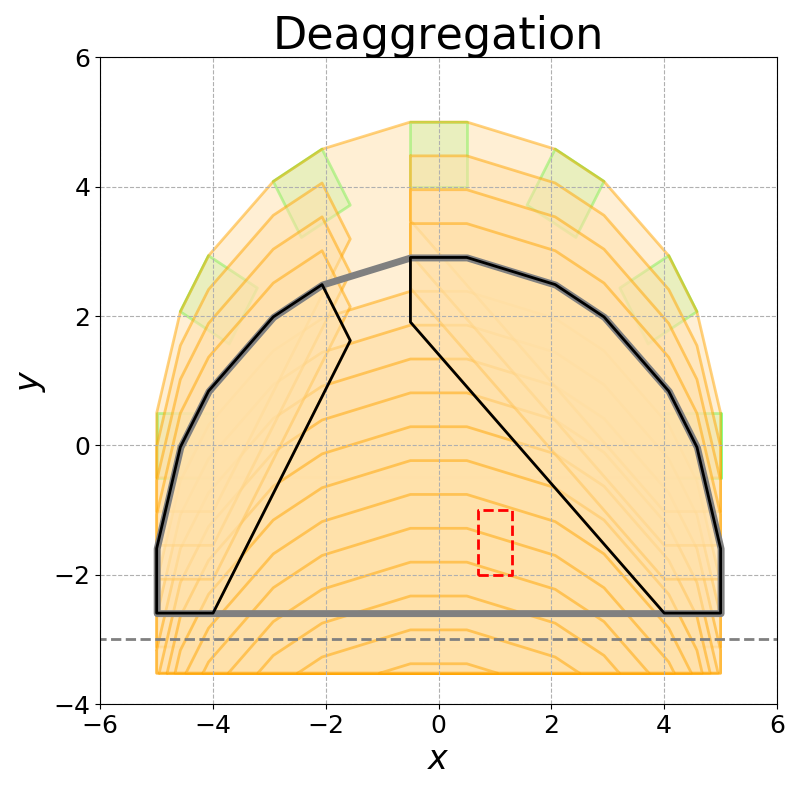
\includegraphics[width=0.8\columnwidth]{images/deagg.png}}
\caption{The deaggregation process is shown for a two-mode system. Upon reaching an error mode (red dotted region), the fully aggregated set of states (gray large region), is split in half (two black regions), which no longer contain error states. A video of the complete computation is available online at \url{https://youtu.be/SDzGKDBq5tM}.}
\label{fig:deagg}
\end{figure}


To overcome the above mentioned challenges, we develop new aggregation and deaggregation techniques. Our technique works the following way. 
First, while handling discrete transitions, we perform aggregation for all the sets in the $queueStars$ that go to the same mode. 
%
The resultant star is tagged as an \textsf{aggregate} and the reachable set computation continues where the sets are tagged as \textsf{aggregate}. 
%
This way of computing the reachable set will result in a conservative overapproximation.
%
If one of the sets in the computation overlaps with the unsafe set $U$, we check if the set is tagged as \textsf{aggregate}.
%
If so, then we go to the initial set in the location and perform deaggregation and recompute the reachable set.
%
Hence, we perform counterexample guided deaggregation.
%
Our algorithm terminates after we find either a counterexample for safety specification or prove that the overapproximation of the reachable set does not overlap with unsafe set.

One of the advantages of generalized stars is that it allows for easy aggregation and deaggregation. 
%
Additionally, leveraging the data structure of generalized stars, we avoid computing the entire reachable set, but only compute the specific sections of the reachable set that are useful for safety verification.
%
To keep track of the recomputations, we maintain a data structure called aggregated directed acyclic graph (AGGDAG).


\subsection{Aggregation Using Generalized Stars}
\label{sec:aggStars}

In this section, we present the advantages of using generalized stars in aggregation and deaggregation. 
%

\begin{lemma}
\label{lem:agg}
Consider stars $S_1 \deq \tup{c, V, P_1}$, $S_2 \deq \tup{c, V, P_2}$, $\ldots$, $S_m \deq \tup{c, V, P_m}$ where the center and the basis vectors for all the stars is the same.
%
A star $S' \deq \tup{c, V, P'}$ is an overapproximation of the union, i.e., $S_1 \cup S_2 \cup \ldots \cup S_m \subseteq S'$, if and only if $(P_1 \vee P_2 \vee P_k) \Rightarrow P'$.
\end{lemma}
\begin{proof}
Trivially follows from the definition of generalized stars.
\end{proof}

In this paper, since all the stars we encounter have predicates that are conjunctions of linear constraints, our overapproximation is also a predicate which is a conjunction of linear constraints. We present a template based and a convex hull based method for aggregation.

\subsubsection{Template Based Aggregation}
%
% To compute the predicate $P'$, we perform a template based method. 
%
For each location, a set of template directions $c_1^{T}, c_2^{T}, \ldots, c_{l}^{T}$ are provided by the user and the predicate $P'$ is determined by selecting the appropriate values of $d_1, d_2, \ldots, d_l$ such that the condition $(P_1 \vee P_2 \vee P_k) \Rightarrow P'$ is satisfied where $P' \deq (c_1^{T}\alpha \leq d_1) \wedge (c_2^{T}\alpha \leq d_2) \wedge \ldots \wedge (c_l^{T}\alpha \leq d_l)$. 

For computing $d_j$, $1 \leq j \leq l$, we solve $m$ linear programming problems. $d_j^i$ is the maximum value of $c_j^T x$ in $P_i$. That is, $d_j^1 = \mathsf{max}~ c_j^T x~ \mathsf{given} P_1$. Similarly, $d_j^2 = \mathsf{max}~ c_j^T x~ \mathsf{given} P_2$. Similarly we compute $d_j^3, \ldots, d_j^l$. The value of $d_j = \mathsf{max} \{d_j^1, d_j^2, \ldots, d_j^l\}$.

\begin{algorithm}[h!]
\SetKwInOut{Input}{input}\SetKwInOut{Output}{output}\SetKw{Return}{return}
\Input{Predicates $P_1, P_2, \ldots, P_m$, template directions $c_1^{T}, c_2^{T}, \ldots, c_l^{T}$.}
\Output{Predicate $P'$ such that $(P_1 \vee \ldots \vee P_m)\Rightarrow P'$.}
\For{each template direction $c_j^{T}$}{
    \For{each star $S_i$}{
        $d_{j}^{i} \gets \mathsf{max} c_j^T \alpha given P_i(\alpha) = \top$\;
    }
    $d_j \gets \mathsf{d_j^1, \ldots, d_j^m}$\;
}

{\bf return} $P' \deq (c_1^T \alpha \leq d_1) \wedge (c_2^T \alpha \leq d_2) \wedge \ldots \wedge (c_l^{T} \alpha \leq d_l)$\;
\caption{Algorithm that computes bounded time simulation equivalent reachable set.}
\label{alg:algoHybrid}
\end{algorithm}



\subsubsection{Convex Hull Aggregation}
